\documentclass[12pt]{article}
\usepackage{url}
\usepackage{graphicx}

%opening
\title{ --The journey of the Ray-tracer -- }
\author{Diego Sebastian Montoya Rodríguez}

\begin{document}
	
	\maketitle
	\vspace{10pt} % Espacio entre el título y la imagen
	
	\begin{figure}[h]
		\centering
		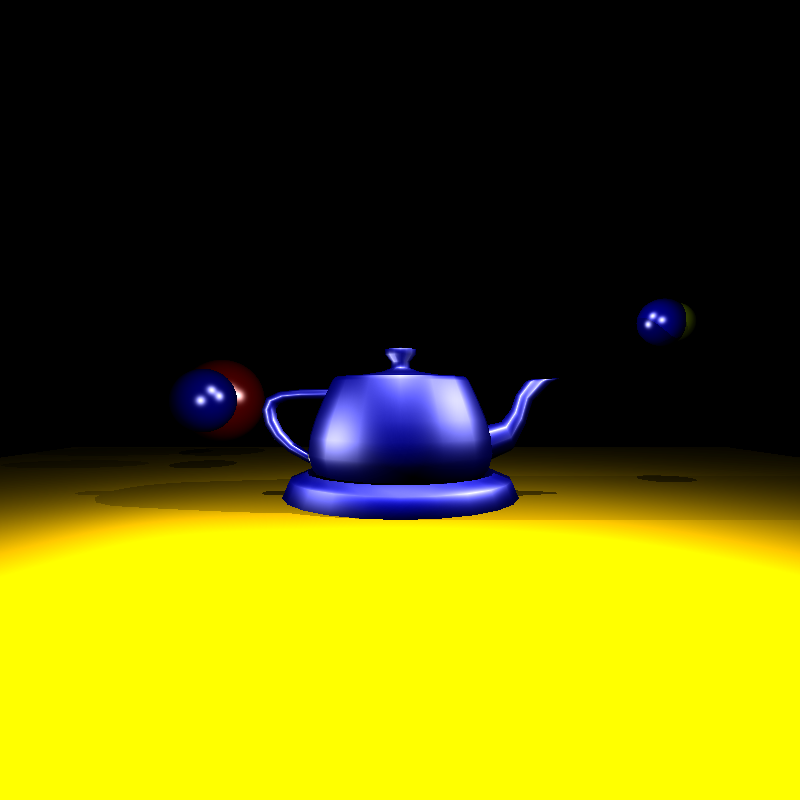
\includegraphics[width=0.6\textwidth]{image7.png}
		\caption{Blinn-Phong image.}
		\label{fig:ejemplo}
		
	\end{figure}
	\pagebreak
	\section{Creation}
	
	The process of making the Ray-tracer was a long journey, but at the same time, it was fun. Finding information about concepts like reflection and refraction, and then implementing them and gradually seeing my program being able to do more and more things, was completely amazing. Honestly, at the beginning of the semester, I was very afraid of this subject, but thanks to the support of my professor and classmates, this class became one of my favorites this semester.\\
	
	When we started the Ray-tracer, we had nothing. We began with a blank file and a bit of theory that gave us an idea of how this ray-tracing system worked. Seeing so many mathematical formulas and knowing I would have to translate them into code overwhelmed me a bit, as I had no idea how I was going to do it. Our first version of the Ray-tracer was a blob model, which only accepted user-created circles and drew the shadow of that circle. When I opened the first file to start programming this version, seeing a blank file that somehow had to become a functional Ray-tracer was shocking; I didn’t know how I was going to do it. Subsequently, we added our first polygon, a triangle. Again, seeing more formulas on the screens scared me a bit, but thanks to this, we could now implement 3D figures. The next step was to add our .obj file reader to import 3D models. Little by little, the Ray-tracer was growing alongside us.\\
	
	At this point, we could import 3D .obj type objects for our Ray-tracer, but it was missing something to really stand out, and that element was lights and shadows. We started with a point light and a directional light, which greatly enhanced our renders. Subsequently, we integrated various things like smooth shadows and light fall-off. It was right in this class that we saw the “SAFETY NET IS OFF” message, indicating that we would no longer receive the kind of help we had been getting up to this point. I remember that upon seeing this, I didn’t feel as scared; on the contrary, I felt excited because the real challenge was beginning.\\
	
	
	
	Now, being on our own, we had to find information about what we needed on our own. The three challenges to tackle were: “Blinn-Phong reflection,” reflection, and refraction. For all three, I had to review a large number of internet pages and videos to first understand the physics and mathematics behind each one to be able to implement it in my Ray-tracer. After a large number of compilation errors and tests, I managed to produce the first render with all the requirements. My version 1.\\
	
	The biggest challenges when creating my Ray-tracer were finding information and knowing how to adapt this information into the code. Additionally, I personally struggled at the beginning, but as we progressed and gained experience, it became easier and easier to accomplish.\\
	
	
	
	
	
	
	
	\section{Process}
	
	\begin{figure}[h]
		\centering
		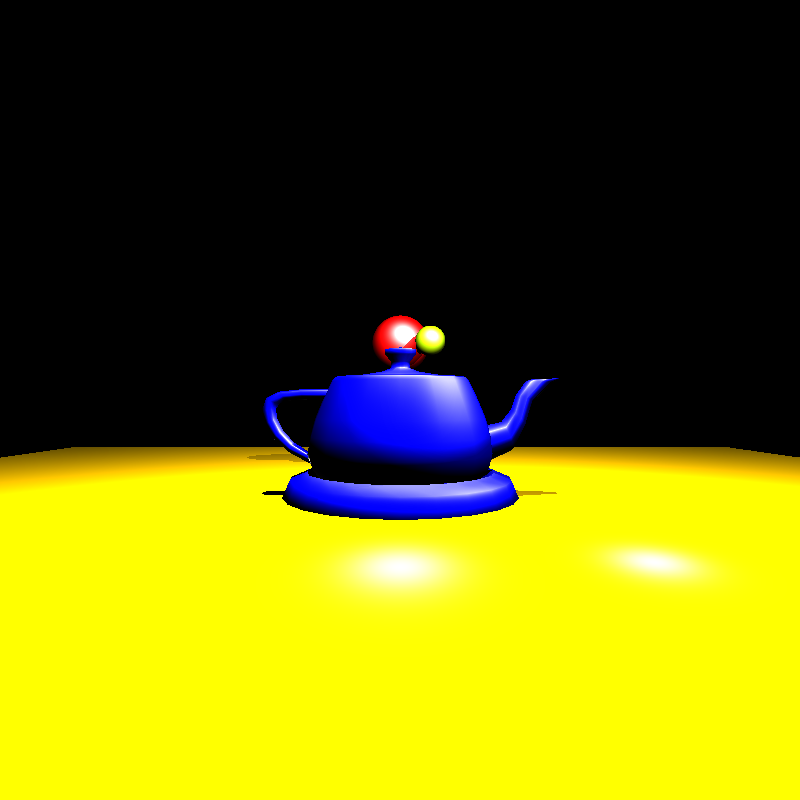
\includegraphics[width=0.6\textwidth]{image.png}
		\caption{First image with Blinn - Phong.}
		\label{fig:image1}
	\end{figure}
	
	\begin{figure}[h]
		\centering
		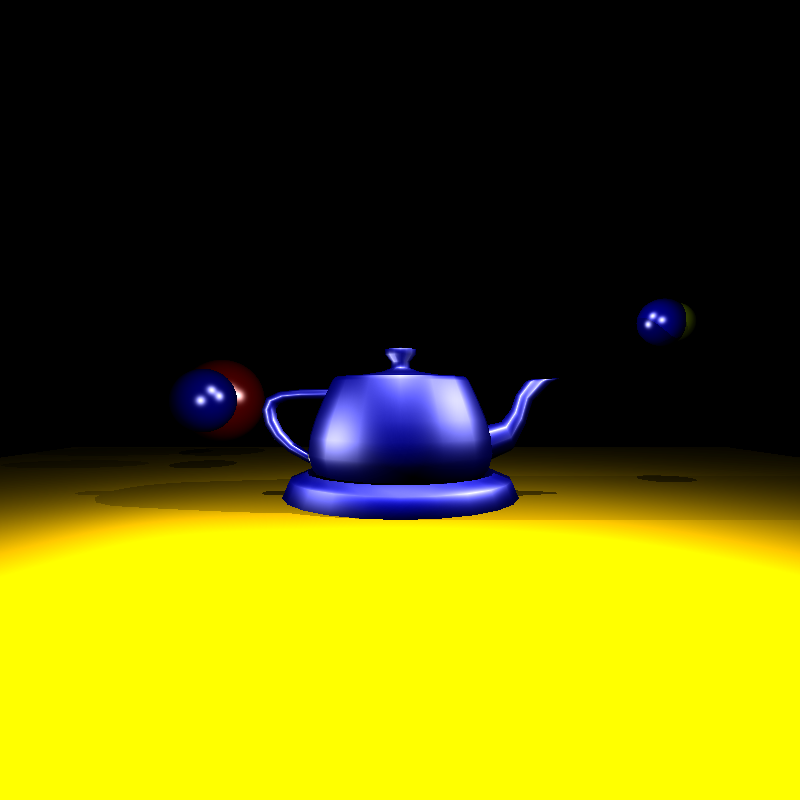
\includegraphics[width=0.6\textwidth]{image7.png}
		\caption{Improved Blinn - Phong.}
		\label{fig:image2}
	\end{figure}
	
	\begin{figure}[h]
		\centering
		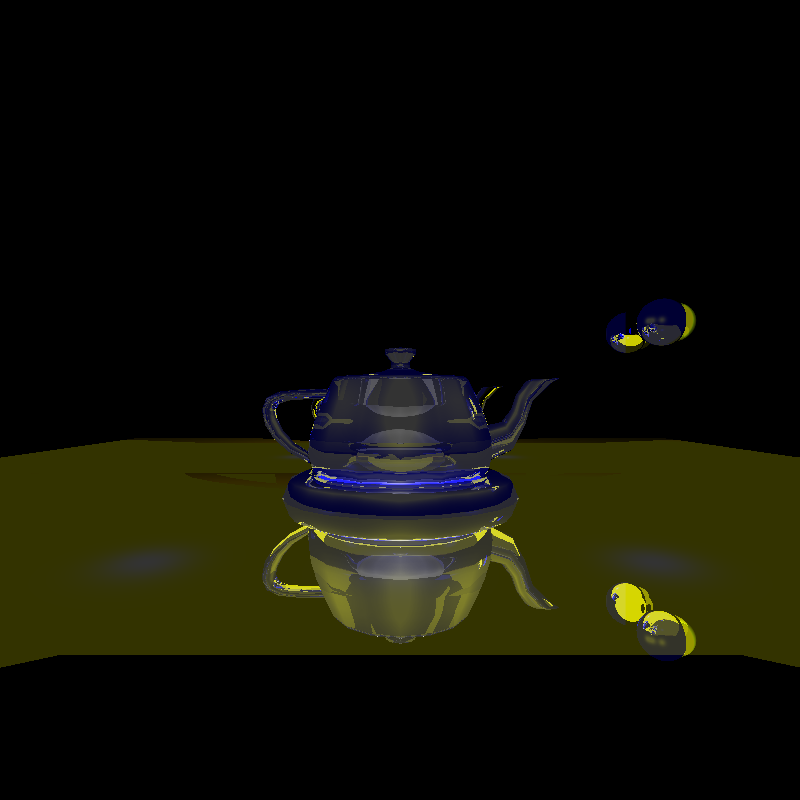
\includegraphics[width=0.6\textwidth]{image12.png}
		\caption{First image with reflection.}
		\label{fig:image3}
	\end{figure}
	
	\begin{figure}[h]
		\centering
		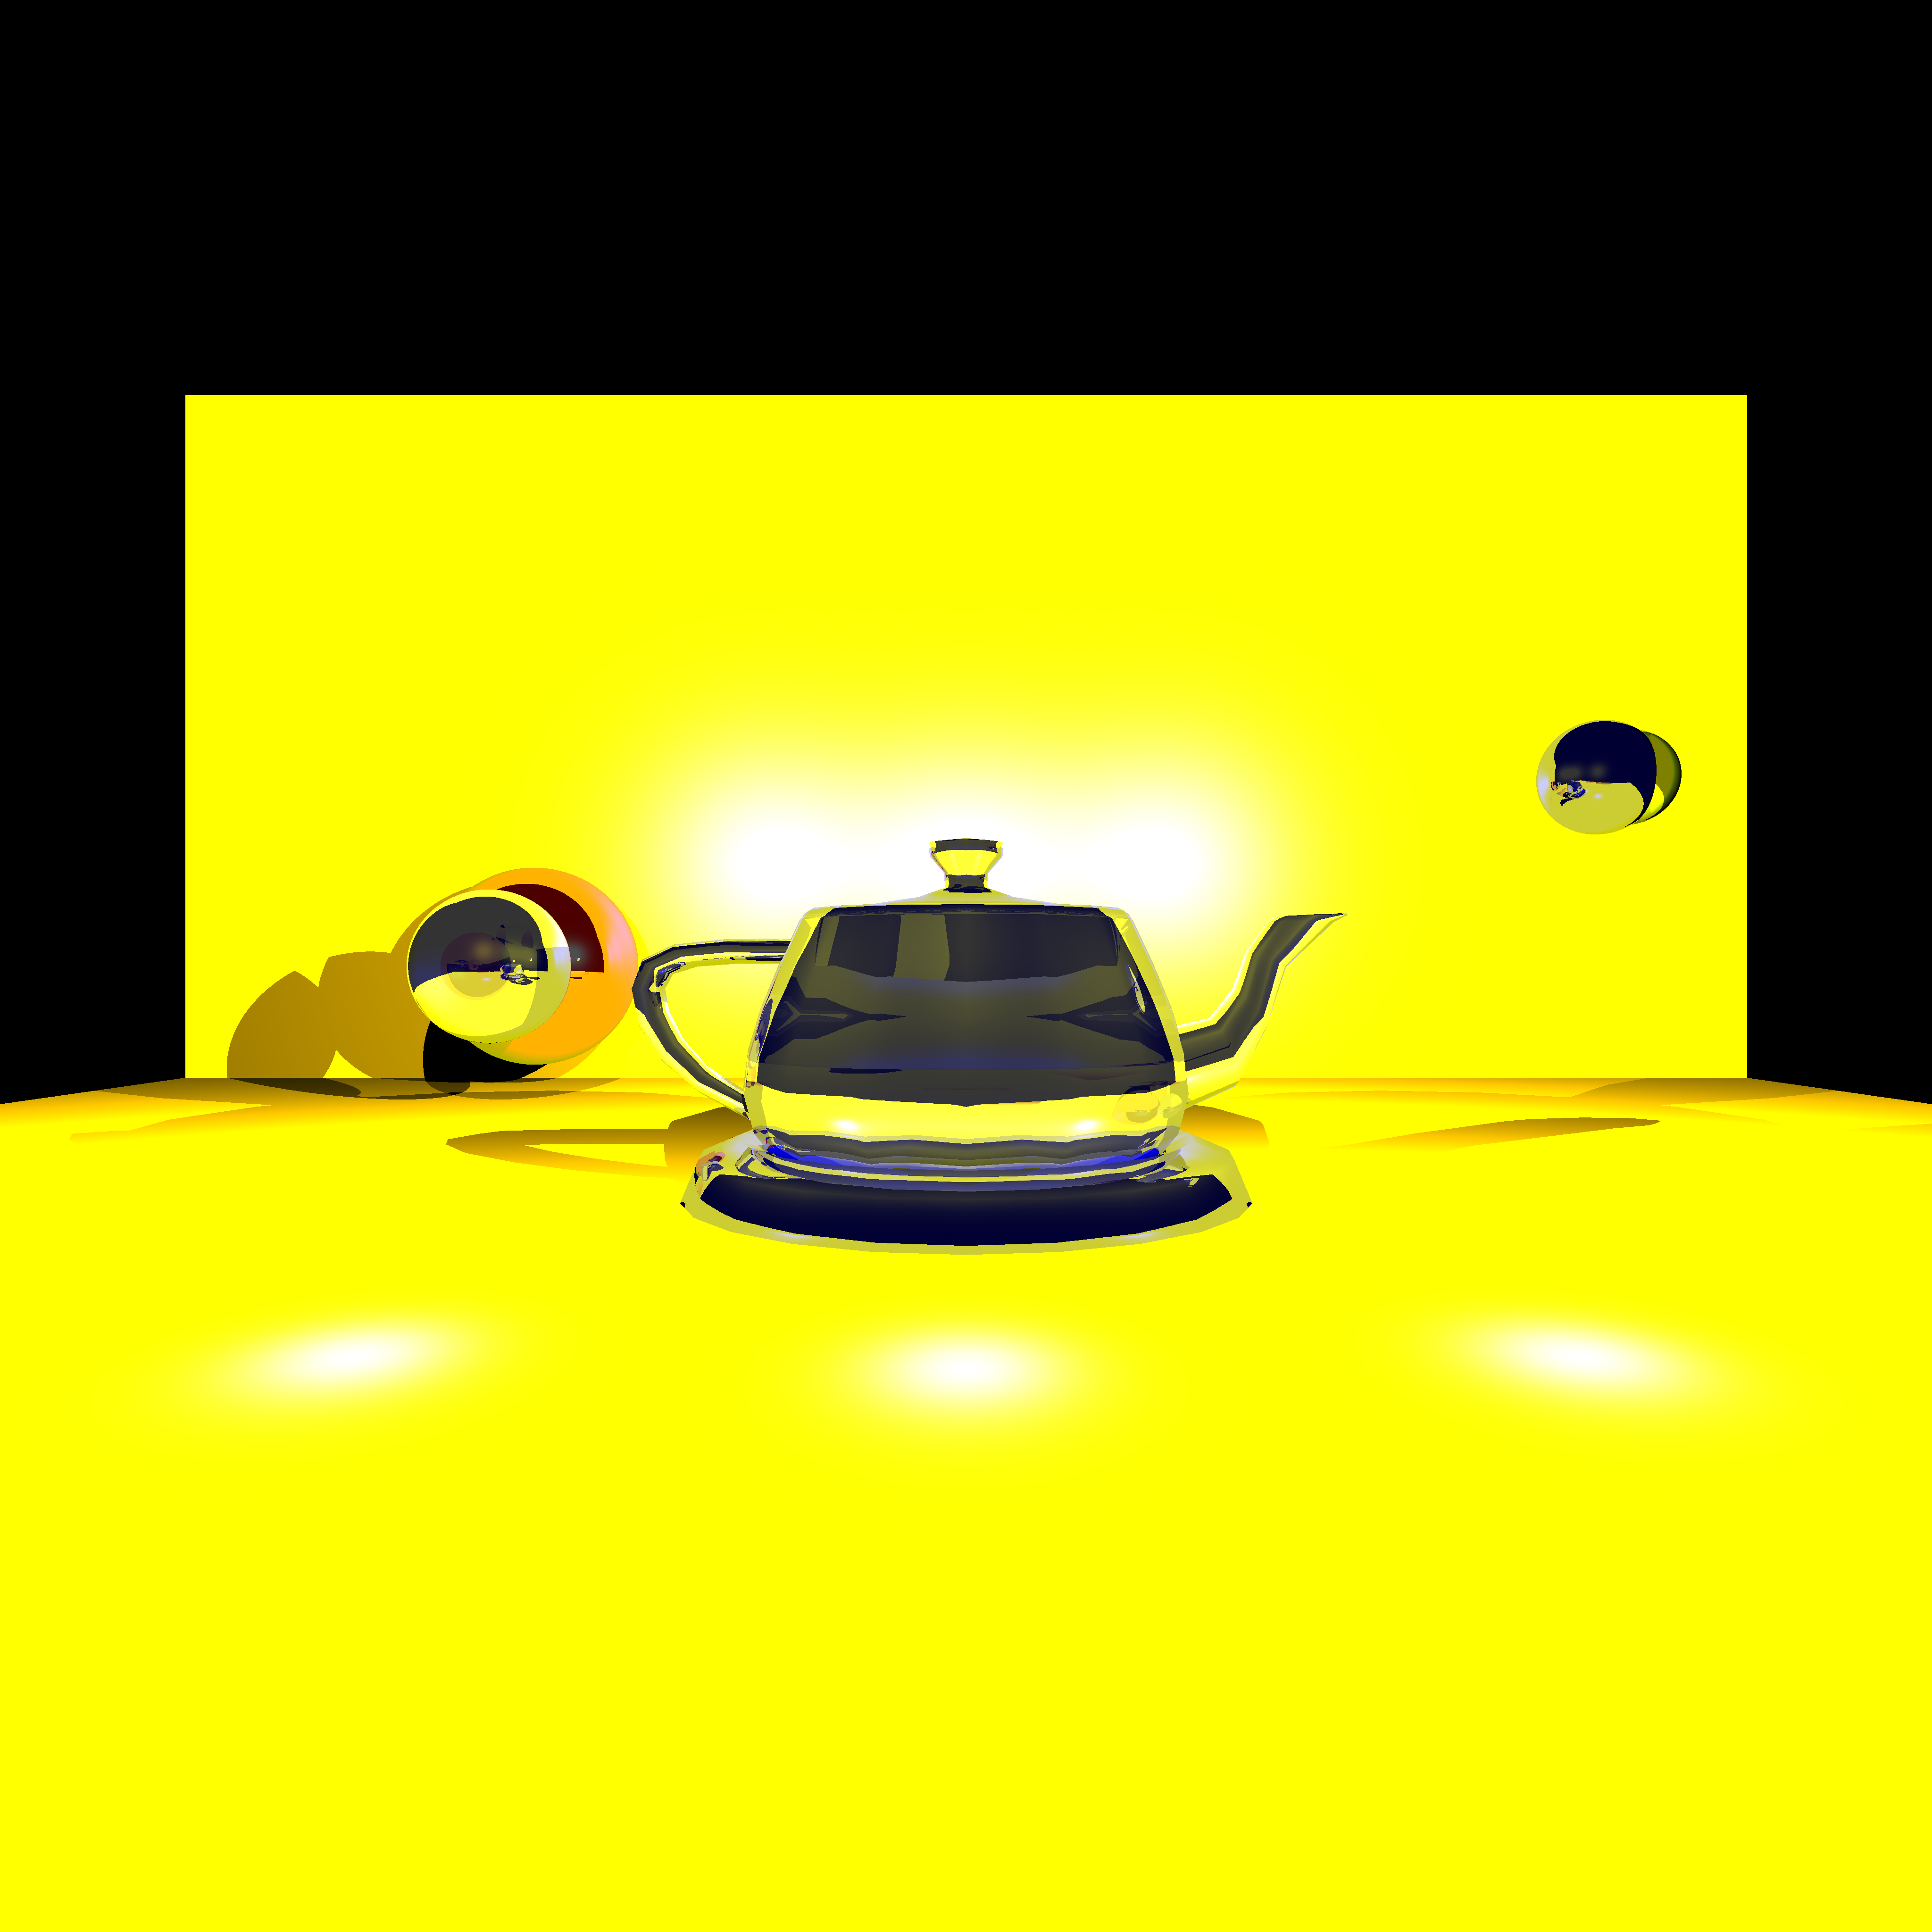
\includegraphics[width=0.6\textwidth]{image19.png}
		\caption{First image with reflection and refraction.}
		\label{fig:image4}
	\end{figure}
	
	\begin{figure}[h]
		\centering
		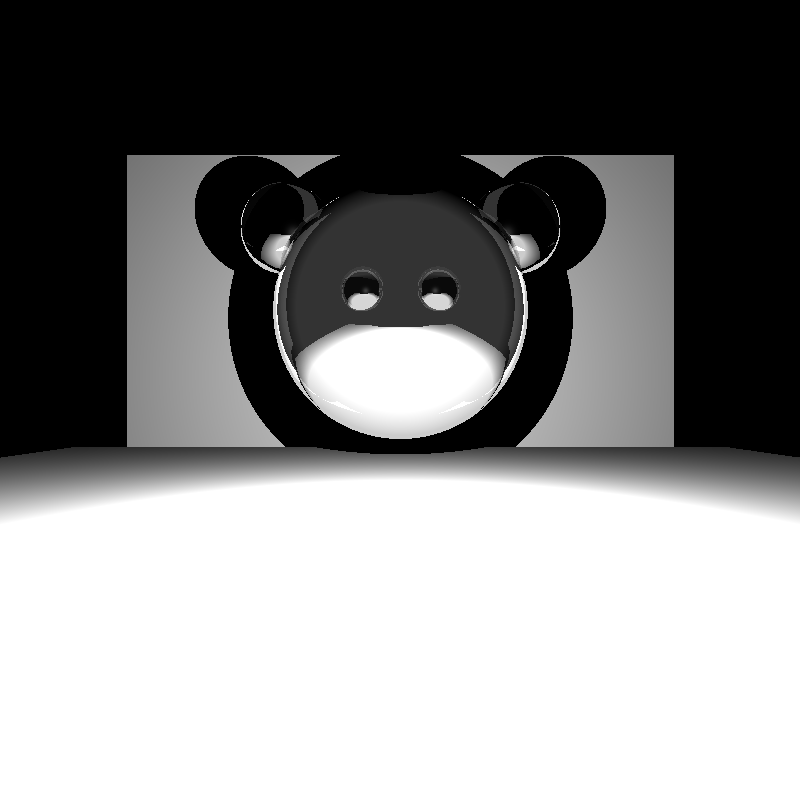
\includegraphics[width=0.6\textwidth]{image20.png}
		\caption{First idea of render.}
		\label{fig:image5}
	\end{figure}
	
	% Fuerza a LaTeX a procesar todas las figuras pendientes antes de la nueva sección
	\clearpage
	
	\section{Final renders}
	
	\begin{figure}[h]
		\centering
		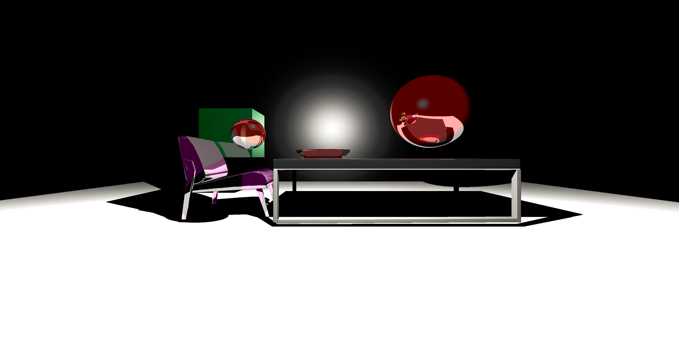
\includegraphics[width=0.6\textwidth]{FINAL1.png}
		\caption{Final render.}
		\label{fig:image6}
	\end{figure}
	
	This is my first 4k render. In the scene, there's a dining area, however, there's only a single chair and plate. This render tells us how we can feel lonely. The red sphere above the chair represents us, while the larger one and the cube represent our thoughts; that's why they are much simpler figures than the rest, such as the chair, table, and plates. This render tells us that even when we are alone, we have ourselves, with a light that strongly impacts on a black plane behind to remind us that this light will always be there because that light is our own soul.\\
	
	\begin{figure}[h]
		\centering
		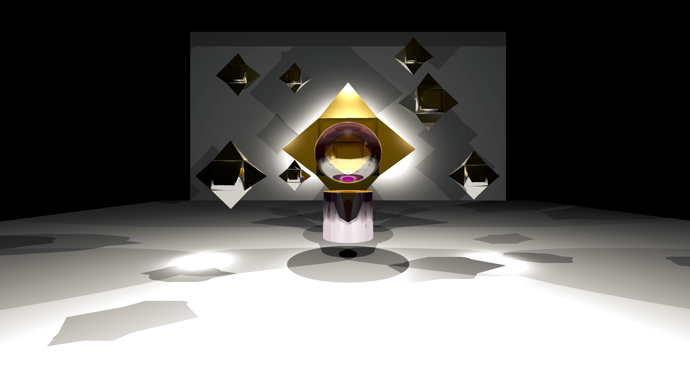
\includegraphics[width=0.6\textwidth]{FINAL2.png}
		\caption{Another final render.}
		\label{fig:image7}
	\end{figure}
	
	This second render represents dreams. The pillar and the sphere represent us; it is surrounded by stars, and in the background, there is a dark void representing the night.\\
	
	\begin{figure}[h]
		\centering
		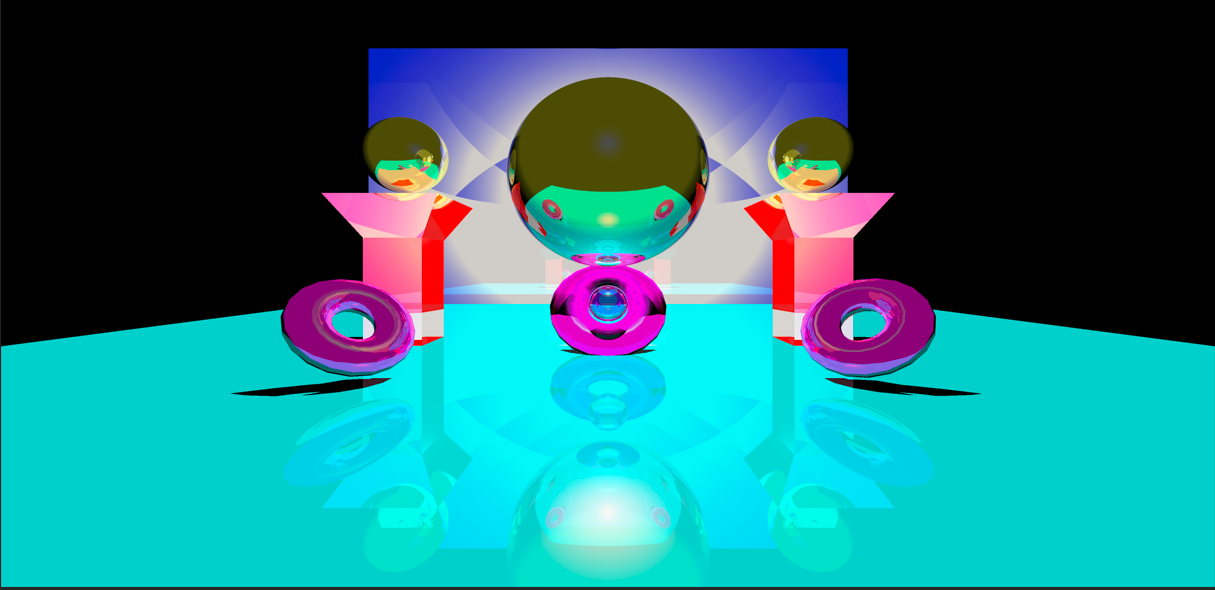
\includegraphics[width=0.6\textwidth]{FINAL3.png}
		\caption{Another final render.}
		\label{fig:image7}
	\end{figure}
	
	The third render represents beach days with very vibrant and bright colors. The sphere represents the Sun, and the ground represents a pool with the donuts symbolizing lifebuoys. The sphere represents us, reminding us of those moments when we were young and went to the beach.
	\section{Self evaluation}
	Does it have unnecessary code? (400 pts) - correct
	
	Does it properly uses OOP? (600 pts) -correct
	
	Is the code reusable? (1,000 pts) - correct
	
	Is the code flexible? (1,000 pts) - correct
	
	Does it have bugs? (800 pts) - minor
	
	Is the code scalable? (800 pts) -minor
	
	Does it have comments? (800 pts) - incorrect
	
	Is the code a huge mess or neat? (1,000 pts) - minor
	
	\section{References}
	
	
	The Organic Chemistry Tutor (2020). Refraction of Light. Retrieved from: \url{https://www.youtube.com/watch?v=ON1QGqB6vxg}\\
	
	Vince, J. (2017). Mathematics for Computer Graphics. Springer.
	
	
	
	
	
	
	
	
	
	
	
	
	
\end{document}
